\documentclass[a4paper,10pt,english]{article}
\usepackage[utf8]{inputenc}
%\usepackage[norsk]{babel}
% Standard stuff
\usepackage{amsmath,graphicx,varioref,verbatim,amsfonts,geometry,grffile}
% colors in text
\usepackage[usenames,dvipsnames,svgnames,table]{xcolor}
% Hyper refs
\usepackage[colorlinks]{hyperref}
\usepackage{flafter}
\usepackage{float}
\usepackage{placeins}
\usepackage{fancyvrb}
\usepackage{comment}
\usepackage{csquotes}

%latex graphics
\usepackage{tikz}
\usetikzlibrary{arrows, decorations.pathmorphing}


% Document formatting
\setlength{\parindent}{0mm}
\setlength{\parskip}{1.5mm}

%Color scheme for listings
\usepackage{textcomp}
\definecolor{listinggray}{gray}{0.9}
\definecolor{lbcolor}{rgb}{0.9,0.9,0.9}

%Listings configuration
\usepackage{listings}
%Hvis du bruker noe annet enn python, endre det her for å få riktig highlighting.
\lstset{
	backgroundcolor=\color{lbcolor},
	tabsize=4,
	rulecolor=,
	language=python,
        basicstyle=\scriptsize,
        upquote=true,
        aboveskip={1.5\baselineskip},
        columns=fixed,
	numbers=left,
        showstringspaces=false,
        extendedchars=true,
        breaklines=true,
        prebreak = \raisebox{0ex}[0ex][0ex]{\ensuremath{\hookleftarrow}},
        frame=single,
        showtabs=false,
        showspaces=false,
        showstringspaces=false,
        identifierstyle=\ttfamily,
        keywordstyle=\color[rgb]{0,0,1},
        commentstyle=\color[rgb]{0.133,0.545,0.133},
        stringstyle=\color[rgb]{0.627,0.126,0.941}
        }
        

\begin{document}
\title{Solutions to exercise in part 2C}
%\author{Johan Andreas Fløisand}
\date{}
\maketitle
\tableofcontents
\clearpage

\addcontentsline{toc}{section}{Usefull formulas and constants}
\section*{Usefull formulas and constants}

\subsection*{Constants}
The following constants may be used:
\begin{itemize}
\item Mass of the Earth:      $M_{\text{Earth}}=5.972\cdot10^{24}\,kg$ 
\item Mass of the sun:        $M_{\text{sun}}=1.989\cdot10^{30}\,kg$
\item Radius of the Earth:    $r_{\text{Earth}}=6371\,km$
\item Radius of the sun:      $r_{\text{sun}}=695\,508\,km$
\item Speed of light:         $c=299\,792\,458\,m/s$
\item Gravitational constant: $G=6.67408\cdot10^{-11}\,\frac{m^{3}}{kg\,s^{2}}$
\end{itemize}

\subsection*{Line elements}
The Schwawrzschild line element is given by:

\begin{equation}\label{eq:schwarzschild}
\Delta s^{2}=\left(1-\frac{2M}{r}\right)\Delta t^{2}-\frac{\Delta r^{2}}{1-\frac{2M}{r}}-r^{2}\Delta\phi^{2},
\end{equation}

where $M$ is the mass of the central mass at $r=0$ (usually a black hole, a star or a planet), $r$ is the Schwarzschild radius (see lecture note 2C if you do not remember this), $\Delta t$ is the difference in time, $\Delta r$ is the difference in radial position and $\Delta\phi$ is the difference in the angular position between two events.
\\
This equation tells us that the intervall $\Delta s^{2}$ between two events is allways equal for all frames of referance.
\\
\\
If we are dealing with a local inertial frame (see lecture note 2C if you do not remember what this is), we are allowed to use the Lorentz line element:

\begin{equation}\label{eq:lorentz}
\Delta s^{2}=\Delta t^{2}-\Delta x^{2}=\Delta t^{2}-\Delta r^{2}-r^{2}\Delta\phi^{2},
\end{equation}

where $\Delta x$ is the difference in $x$-position and all other variables are the same as in the Schwarzschild line element. As above, $\Delta s^{2}$ between two events is equal for all observers.


\subsection*{Change of units}

In the theory of relativity we will use natural unit. That is, we want to measure time and mass in meters. We converte between mass in kilos and meters as follows:

\begin{equation}\label{eq:kg_to_m}
\frac{M_{m}}{M_{kg}}=\frac{G}{c^{2}}\left(\approx\frac{6.67408\cdot10^{-11}\,m^{3}kg^{-1}s^{-2}}{(299\,792\,458\,m/s)^{2}}\approx7.4259\cdot10^{-28}\right)
\end{equation}

Here $M_{m}$ and $M_{kg}$ the mass of the object in question in meters and kilos respectively, $G$ is the gravitational constant and $c$ is the speed of light.
%$\frac{G}{c^{2}}\approx\frac{6.67408\cdot10^{-11}\,m^{3}kg^{-1}s^{-2}}{(299\,792\,458\,m/s)^{2}}\approx7.4259\cdot10^{-28}$
\\
\\
To converte between time in seconds and meters we do like this:
 
\begin{equation}\label{eq:s_to_m}
t_{s}\cdot c=t_{m}
\end{equation}

Here $t_{s}$ and $t_{m}$ is time in seconds and meters respectively and $c$ is the speed of light.


\subsection*{Time and length differance between observers}

In lecture note 2C we have deduced the following relation between the time and length measured by the shell and far-away observer:

\begin{equation}\label{eq:shell_time}
\Delta t_{\text{shell}}=\Delta t\sqrt{1-\frac{2M}{r}},
\end{equation}
and
\begin{equation}\label{eq:shell_length}
\Delta r_{\text{shell}}=\frac{\Delta r}{\sqrt{1-\frac{2M}{r}}}
\end{equation}

Here $\Delta t_{\text{shell}}$ and $\Delta t$ is the time difference measured by the shell and far-away observer respectively, $\Delta r_{\text{shell}}$ and $\Delta r$ is the difference in radial position measured by the shell and far-away observer respectively, $M$ is the mass of the central mass and $r$ is the Schwarzschild radius.

\subsection*{Conservation laws}
In lecture note 2C we are given the following consevation laws:
\\
Energy per mass

\begin{equation}\label{eq:E/m}
\frac{E}{m}=\left(1-\frac{2M}{r}\right)\frac{dt}{d\tau}=\text{constant},
\end{equation}

where $E$ and $m$ is the energy and mass of the object, $M$ is the mass of the central mass, $r$ is the Schwazscild radius, $dt$ the time difference measured by the far-away observer and $d\tau$ is the proper time of the object.

Angular momentum per mass

\begin{equation}\label{eq:L/m}
\frac{L}{m}=r^{2}\frac{d\phi}{d\tau}=\gamma_{\text{shell}}rv_{\phi}=\text{constant},
\end{equation}

where $L$ is the angular momentum, $m$ is the mass of the object, $r$ is the Schwarzschild radius, $d\phi$ is the angular difference measured by the far-away observer, $d\tau$ is the proper time of the object, $\gamma_{\text{shell}}=\frac{1}{\sqrt{1-v_{\text{shell}}^{2}}}$ where $v_{\text{shell}}$ is the velocity of the object measured by a shell observer and $v_{\phi}$ is the angular velocity of the object measured by the far-away observer.

\newpage








\addcontentsline{toc}{section}{Exercise 2C.1}
\section*{Exercise 2C.1}


We are observing a laser with frequency $\nu_{\text{shell}}=1/\Delta t_\text{shell}$, measured by a shell observer at a distance $r$ from a central mass $M$, and $\nu^{\prime}=1/\Delta t^{\prime}$, measured by a far-away observer (when the laser reaches him). $\Delta t^{\prime}$ and $\Delta t_\text{shell}$ are the difference between two peaks of the electromagnetic wave of the laser.

\begin{enumerate}

\item We want to find the relation between the two time differences. In lecture note 2C we derived a relation between the time measured by a shell and far-away observer (equation \ref{eq:shell_time}). We derived this equation assuming $\Delta r=0$, $\Delta\phi=0$ and that the shell observer was in a local inertial frame so that $\Delta s^{2}=\Delta\tau^{2}=\Delta t_{\text{shell}}$. 
%, which is valid for $\Delta r_{shell}\approx0$ and $\Delta \phi_\text{shell}=0$. 
Since the distance between two peaks on an electromagnetic wave is very small (if we exclude radio waves), the wave is only moving in radial direction and we can think of an observer \textquote{on} the wave as a shell observer in a local inertial frame, we are allowed to use equation \ref{eq:shell_time} which gives us 

\[\Delta t^{\prime}=\frac{\Delta t_{\text{shell}}}{\sqrt{1-\frac{2M}{r}}}\]

\item We should now be able to show the gravitational ``Doppler" formula. We know that the relation between wave length and frequency is $\lambda=\frac{c}{\nu}=\frac{1}{\nu}$, since $c=1$ in our relativistic units (where $\lambda$ and $\nu$ is the wave length and frequency of an electromagnetic wave). Using that frequency is given by $\nu=\frac{1}{\Delta t}$, we get (remember that want to find an expression for $\frac{\Delta \lambda}{\lambda}$)

\begin{align*}
\frac{\Delta \lambda}{\lambda_{\text{shell}}}&=\frac{\lambda^{\prime}-\lambda_{\text{shell}}}{\lambda_{\text{shell}}}=\frac{\lambda^{\prime}}{\lambda_{\text{shell}}}-1=\frac{1/\nu^{\prime}}{1/\nu_{\text{shell}}}-1\\
&=\frac{\Delta t^{\prime}}{\Delta t_{\text{shell}}}-1=\frac{\Delta t_{\text{shell}}}{\sqrt{1-\frac{2M}{r}}}\frac{1}{\Delta t_{\text{shell}}}-1\\
&=\frac{1}{\sqrt{1-\frac{2M}{r}}}-1
\end{align*}

In the second line we use the relation we found above (equation\ref{eq:shell_time}).
  
\item To show the relation $\frac{\Delta \lambda}{\lambda_{\text{shell}}}=\frac{M}{r}$ when $r\gg2M$, we will create a Taylor expansion. We define $f(x)=\frac{1}{\sqrt{1-x}}$. In other words, if we choose $x=\frac{2M}{r}$ we have

\[\frac{\Delta \lambda}{\lambda_{\text{shell}}}=\frac{1}{\sqrt{1-\frac{2M}{r}}}-1=f(x)-1\]

We start by finding the derivative.

\begin{align*}
f^{\prime}(x)&=\left[(1-x)^{-1/2}\right]^{\prime}=\frac{-1}{2}(1-x)^{-3/2}(-1)=\frac{1}{2}(1-x)^{-3/2} &&\Rightarrow&& f^{\prime}(0)&=\frac{1}{2}
\end{align*}  

This means that we can write the first order Taylor expasion for $f(x)$ (this will be a good approximation for $r\gg 2M$.

\begin{equation*}
\frac{1}{\sqrt{1-x}}=f(x)\approx T_{1}f(x)=f(0)+xf^{\prime}(0)=1+\frac{1}{2}x
\end{equation*}

Inserting our newfound Taylor expansion into the relativistic \textquote{Doppler} formula we find

\begin{align*}
\frac{\Delta \lambda}{\lambda_{\text{shell}}}&=\frac{1}{\sqrt{1-\frac{2M}{r}}}-1\approx T_{1}f(2M/r)-1=f(0)+\frac{2M}{r}f^{\prime}(0)-1=1+\frac{1}{2}\frac{2M}{r}-1\\
&=\frac{M}{r}
\end{align*}


\item We will now study how the relativistic doppler formula acts on the light from the sun. We will assume that the wave length of the light from the sun is at maximum $\lambda_{\text{max}}=500\,nm$.

\begin{enumerate}

\item First we need to find the mass of our sun in meters. Equation \ref{eq:kg_to_m} tells us how to converte from kilos to meters.

\[M_{m}=\frac{G}{c^{2}}M_{kg}=7.4259\cdot10^{-28}\,m/kg\cdot2\cdot10^{30}\,kg\approx1485.18\,m\]

\item we can now find the ratio $M/r$ for the sun (the radius of the sun is listed under constants). 

\[\frac{M}{r}\approx\frac{1485.18\,m}{695\,508\cdot10^{3}\,m}\approx2.1354\cdot10^{-6}\]

\item We now want to find the redshift measured by a far-away observer. Since $\frac{2M}{r}\ll 1$ we are allowed to use our Taylor expansion $\frac{\Delta \lambda}{\lambda}=\frac{M}{r}\approx2.1354\cdot10^{-6}$.
\\
Alternatively we can use the full expression:
\begin{equation*}
\frac{\Delta \lambda}{\lambda}=\frac{1}{\sqrt{1-\frac{2M}{r}}}-1\approx\frac{1}{\sqrt{1-2\cdot2.1354\cdot10^{-6}}}-1\approx2.1354\cdot10^{-6}
\end{equation*}
  
\item The color of the sun observed by a far-away observer will be

\begin{align*}
\frac{\Delta \lambda}{\lambda}&=\frac{\lambda^{\prime}-\lambda_{\text{shell}}}{\lambda_{\text{shell}}}=\frac{1}{\sqrt{1-\frac{2M}{r}}}-1\\
\frac{\lambda^{\prime}}{\lambda_{\text{shell}}}&=\frac{1}{\sqrt{1-\frac{2M}{r}}}\\
\lambda^{\prime}&=\frac{1}{\sqrt{1-\frac{2M}{r}}}\lambda_{\text{shell}}\approx\frac{1}{\sqrt{1-2\cdot2.1354\cdot10^{-6}}}\cdot500\cdot10^{-9}\,m\approx500.001\,nm
\end{align*}

The apparent color of the sun will therefore not change.
  
\item We now want to study how light from a sun-like star is affected by the Earth's gravitational pull (the mass and radius of the Earth are listed under constants). We begin by finding Earth's mass in meters 

\[M_{m,\text{Earth}}=\frac{G}{c^{2}}M_{kg,\text{Earth}}\approx7.4259\cdot10^{-28}\,m/kg\cdot5.972\cdot10^{24}\,kg\approx4.4347\cdot10^{-3}\,m,\]

hence the mass to radius ratio becomes

\[\frac{M}{r}\approx\frac{4.4347\cdot10^{-3}\,m}{6\,371\cdot10^{3}\,m}\approx6.9608\cdot10^{-10}\]
  
\item We are now almost ready to find the Doppler shift caused by the Earth. Notice that we need to redefine who the far-away and shell observer is (the observer on Earth will be the shell observer and the one close to the sun will be the far-away observer). To be consistent, we will therefore switch the places in the Doppler formula (the ratio between the two wave lengths will be the same even if we do not switch the places).

\begin{align*}
\frac{\Delta \lambda}{\lambda^{\prime}}&=\frac{\lambda_{\text{shell}}-\lambda^{\prime}}{\lambda^{\prime}}=\frac{\Delta t_{\text{shell}}}{\Delta t^{\prime}}-1\\
&=\frac{\Delta t_{\text{shell}}}{\Delta t_{\text{shell}}/\sqrt{1-\frac{2M}{r}}}-1=\sqrt{1-\frac{2M}{r}}-1\\
&\approx\sqrt{1-2\cdot6.9608\cdot10^{-10}}-1\approx-6.9608\cdot10^-{10}
\end{align*}

Thus the observed wave length on earth is

\begin{align*}
\frac{\Delta \lambda}{\lambda^{\prime}}&=\frac{\lambda_{\text{shell}}}{\lambda^{\prime}}-1=\sqrt{1-\frac{2M}{r}}-1\\
\lambda_{\text{shell}}&=\lambda^{\prime}\sqrt{1-\frac{2M}{r}}\approx500\,nm\cdot\sqrt{1-6.9608\cdot10^{-10}}\\
&\approx500.000\,nm
\end{align*}
  
\end{enumerate}

\item We are now looking at waves observed from a quasar and we want to find the distance $r$ in terms of $M$. The shell observer will be the observer close to the quasar and the far-away observer will be us on Earth. We are given $\lambda^{\prime}=600\,nm$ and $\lambda_{\text{shell}}=2150\,nm$. Rearranging the the relativistic Doppler formula and putting in numbers, we find:

\begin{align*}
\frac{\Delta \lambda}{\lambda_{\text{shell}}}&=\frac{\lambda^{\prime}}{\lambda_{\text{shell}}}-1=\frac{1}{\sqrt{1-\frac{2M}{r}}}-1\\
1-\frac{2M}{r}&=\left(\frac{\lambda_{\text{shell}}}{\lambda^{\prime}}\right)^{2}\\
\frac{2M}{r}&=1-\left(\frac{\lambda_{\text{shell}}}{\lambda^{\prime}}\right)^{2}\\
r&=\frac{2M}{1-\left(\frac{\lambda_{\text{shell}}}{\lambda^{\prime}}\right)^{2}}\\
r&=\frac{2}{1-\left(\frac{600\,nm}{2150\,nm}\right)^{2}}M\approx2.1689M
\end{align*}

We know from lecture note 2C that the Schwarzschild radius of a black hole is located at $r=2M$. Since the light we measure is is emitted at a distance $r\approx2M$, it would make sence that there is a black hole at the center of the quasar (light closer to the black hole then $r=2M$ will just fall into it).

\item We are now situated at $r=2.01M$ as a shell observer around a black hole with mass $M$. We want to find the Doppler shift from the stars around us. The Doppler formula gives us

\begin{align*}
\frac{\Delta \lambda}{\lambda^{\prime}}&=\frac{\lambda_{\text{shell}}}{\lambda^{\prime}}-1=\sqrt{1-\frac{2M}{r}}-1\\
\lambda_{\text{shell}}&=\lambda^{\prime}\sqrt{1-\frac{2M}{r}}=\lambda^{\prime}\sqrt{1-\frac{2M}{2.01M}}\approx0.0705\lambda^{\prime}
\end{align*}

This means that we would need a telescope that can observe x-rays to look at the different stars.

\end{enumerate}
  








\addcontentsline{toc}{section}{Exercise 2C.2}
\section*{Exercise 2C.2}

We are looking at two shell observers: one close to the black hole far from the black hole. We want to study how they experience time differently.

\begin{enumerate}

\item First we need to find the mass of the black hole in our relativistic units. Equation \ref{eq:kg_to_m} tells us how to convert mass from kilo into meters. 

\[\frac{M_{m}}{M_{kg}}=\frac{G}{c^{2}}\] 

(Check $\ldots$ for solution)

\item Here you have to check MCast for solution. We suggest that you create a similar table to table \ref{table:1}. Note that all times are in your own frame.

  \begin{table}[H]
  \begin{center}
    \begin{tabular}{| l | l | l | l | l | l | l | }
   	\hline
	Time & Wake up & Breakfast & Lunch & Dinner & Brush teeth & Bed \\ \hline
	 $t$ (your schedule) & $t_{1}$ & $t_{2}$ & $t_{3}$ & $t_{4}$ & $t_{5}$ & $t_{6}$ \\ \hline
	 $t^{\prime}$ (partners schedule) & $t^{\prime}_{1}$ & $t^{\prime}_{2}$ & $t^{\prime}_{3}$ & $t^{\prime}_{4}$ & $t^{\prime}_{5}$ & $t^{\prime}_{6}$\\ \hline
	\end{tabular}
    \caption{A table for the different times in your frame.}
    \label{table:1}
  \end{center}
\end{table}


\item Having found the time of your partners routine, you should now converte the time from seconds to meters. Equation \ref{eq:s_to_m} tells us how to do this. 

\[t_{s}\cdot c=t_{m}\] 

(Check $\ldots$ for solution)

\item We know how to converte between time for the shell and far-away observer, but not between different shell observers. We can think of our situation as having two shells: shell 1 (closest to the black hole at a distance $r_{1}$) and shell 2 (furthest away at a distance $r_{2}$). Using the relation between shell and far-away time (equation \ref{eq:shell_time}) we find

\begin{align*}
\Delta t_{\text{shell 1}}=\Delta t\sqrt{1-\frac{2M}{r_{1}}} &&\Rightarrow&& \Delta t=\frac{\Delta t_{\text{shell 1}}}{\sqrt{1-\frac{2M}{r_{1}}}}\\
\Delta t_{\text{shell 2}}=\Delta t\sqrt{1-\frac{2M}{r_{2}}} &&\Rightarrow&& \Delta t=\frac{\Delta t_{\text{shell 2}}}{\sqrt{1-\frac{2M}{r_{2}}}}
\end{align*}

Inserting one into the other we find

\begin{equation*}
\Delta t_{\text{shell 2}}=\Delta t\sqrt{1-\frac{2M}{r_{2}}}=\frac{\Delta t_{\text{shell 1}}}{\sqrt{1-\frac{2M}{r_{1}}}}\sqrt{1-\frac{2M}{r_{2}}}=\frac{\sqrt{1-\frac{2M}{r_{2}}}}{\sqrt{1-\frac{2M}{r_{1}}}}\Delta t_{\text{shell 1}}
\end{equation*}

\item It should now be easy to transforme between the different times with the above formula, but remember that you have the time in meters and not days and hours. To converte back to days and hours we do like this:

\begin{equation*}
t_{\text{hours}}=\frac{t_{s}}{60\cdot60}=\frac{t_{m}\cdot c}{3600}
\end{equation*}

(Check $\ldots$ for solution)

\item \textbf{Slå sammen 5 og 6}

\item Talk with your partner.
  
\end{enumerate}








\addcontentsline{toc}{section}{Exercise 2C.3}
\section*{Exercise 2C.3}

In this exercise we will show that angular momentum per mass is conserved in general relativity, using the principal of maximal aging. The deduction is very similar to those done in the lecture note.

\begin{enumerate}

\item First we want to find an expression for $\Delta\tau_{13}=\Delta\tau_{12}+\Delta\tau_{23}$. We will find $\Delta\tau_{12}$ and $\Delta\tau_{23}$ separately. We know that if we look at a very small movement in space, we can assume that the radius $r$ in the Schwarzschild line element is constant. Since the proper time is always equal to Schwarzschild line element we find

\begin{align*}
\Delta \tau_{12}^{2}&=\Delta s_{12}^{2}=\left(1-\frac{2M}{r_{A}}\right)\Delta t_{12}^{2}-\frac{\Delta r_{12}^{2}}{1-\frac{2M}{r_{A}}}-r_{A}^{2}\Delta \phi_{12}^{2}\\
\Delta \tau_{23}^{2}&=\Delta s_{23}^{2}=\left(1-\frac{2M}{r_{B}}\right)\Delta t_{23}^{2}-\frac{\Delta r_{23}^{2}}{1-\frac{2M}{r_{B}}}-r_{B}^{2}\Delta \phi_{23}^{2}
\end{align*}

Taking the square root we only get the positive solution here since we look at time moving in positive direction. The proper time between position 1 and 3 (since proper time is linear) must be $\Delta \tau_{13}=\Delta \tau_{12}+\Delta \tau_{23}$. Using the expressions we found above we get

\begin{align*}
\Delta \tau_{13}&=\Delta \tau_{12}+\Delta \tau_{23}\\
&=\sqrt{\left(1-\frac{2M}{r_{A}}\right)\Delta t_{12}^{2}-\frac{\Delta r_{12}^{2}}{1-\frac{2M}{r_{A}}}-r_{A}^{2}\Delta \phi_{12}^{2}}+\sqrt{\left(1-\frac{2M}{r_{B}}\right)\Delta t_{23}^{2}-\frac{\Delta r_{23}^{2}}{1-\frac{2M}{r_{B}}}-r_{B}^{2}\Delta \phi_{23}^{2}}
\end{align*}

\item If we now take the derivative of the proper time $\Delta \tau_{13}$ with respect to the angle $\phi_{2}$, the principle of maximal aging tells us that the object will choose the angle which gives the largest proper time. In other words, we want to find the maximum of $\tau_{13}(\phi_{2})$, hence we want to find the value of $\phi_{2}$ such that $\frac{d\tau_{13}}{d\phi_{2}}=0$. \textbf{Hvorfor er dette toppunkt?}%Since time (and therefore especially proper time) is a monotone function, 

\begin{align*}
\frac{d\tau_{13}}{d\phi_{2}}&=\frac{d\tau_{12}}{d\phi_{2}}+\frac{d\tau_{23}}{d\phi_{2}}
=\frac{\sqrt{\left(1-\frac{2M}{r_{A}}\right)\Delta t_{12}^{2}-\frac{\Delta r_{12}^{2}}{1-\frac{2M}{r_{A}}}-r_{A}^{2}\Delta \phi_{12}^{2}}}{d\phi_{2}}+\frac{\sqrt{\left(1-\frac{2M}{r_{B}}\right)\Delta t_{23}^{2}-\frac{\Delta r_{23}^{2}}{1-\frac{2M}{r_{B}}}-r_{B}^{2}\Delta \phi_{23}^{2}}}{d\phi_{2}}\\
&=\frac{1}{2\sqrt{\left(1-\frac{2M}{r_{A}}\right)\Delta t_{12}^{2}-\frac{\Delta r_{12}^{2}}{1-\frac{2M}{r_{A}}}-r_{A}^{2}\Delta \phi_{12}^{2}}}\frac{\left(1-\frac{2M}{r_{A}}\right)\Delta t_{12}^{2}-\frac{\Delta r_{12}^{2}}{1-\frac{2M}{r_{A}}}-r_{A}^{2}(\phi_{2}-\phi_{1})^{2}}{d\phi_{2}}\\
&\;\;\;\;\;+\frac{1}{2\sqrt{\left(1-\frac{2M}{r_{B}}\right)\Delta t_{23}^{2}-\frac{\Delta r_{23}^{2}}{1-\frac{2M}{r_{B}}}-r_{B}^{2}\Delta \phi_{23}^{2}}}\frac{\left(1-\frac{2M}{r_{B}}\right)\Delta t_{23}^{2}-\frac{\Delta r_{23}^{2}}{1-\frac{2M}{r_{B}}}-r_{B}^{2}(\phi_{3}-\phi_{2})^{2}}{d\phi_{2}}\\
&=\frac{1}{2}\frac{1}{d\tau_{12}}\left(\left(1-\frac{2M}{r_{A}}\right)\frac{\Delta t_{12}^{2}}{d\phi_{2}}-\frac{1}{1-\frac{2M}{r_{A}}}\frac{\Delta r_{12}^{2}}{d\phi_{2}}-r_{A}^{2}\frac{(\phi_{2}-\phi_{1})^{2}}{d\phi_{2}}\right)\\
&\;\;\;\;\;+\frac{1}{2}\frac{1}{d\tau_{23}}\left(\left(1-\frac{2M}{r_{B}}\right)\frac{\Delta t_{23}^{2}}{d\phi_{2}}-\frac{1}{1-\frac{2M}{r_{B}}}\frac{\Delta r_{23}^{2}}{d\phi_{2}}-r_{B}^{2}\frac{(\phi_{3}-\phi_{2})^{2}}{d\phi_{2}}\right)\\
&=\frac{1}{2}\frac{1}{d\tau_{12}}(0-0-2r_{A}^{2}d\phi_{12})\cdot1+\frac{1}{2}\frac{1}{d\tau_{23}}(0-0-2r_{B}^{2}d\phi_{23})\cdot(-1)\\
&=-\frac{1}{2}\frac{1}{d\tau_{12}}(2r_{A}^{2}d\phi_{12})+\frac{1}{2}\frac{1}{d\tau_{23}}(2r_{B}^{2}d\phi_{23})
\end{align*}

Setting this equal to zero and equation we find

\begin{equation*}
\frac{r_{A}^{2}d\phi_{12}}{d\tau_{12}}=\frac{r_{B}^{2}d\phi_{23}}{d\tau_{23}}
\end{equation*}

\item What we have found is true for all intervalls $[a_{0},a_{1}]$ small enough. Thus if the intervall was larger, for instance $[a=a_{0},a_{n}=b]$, we could separate it to $n$ small enough intervalls so that the equation over holds for every intervall. By the principal of induction we get $\frac{d\phi_{ab}}{d\tau_{ab}}r_{ab/2}^{2}=\text{constant}$. In other words, 

\[\frac{r^{2}d\phi}{d\tau}=\text{constant}\] 

regardless of the intervall.

\item We remember from celest mechanics that angular velocity, measured by the shell observer, is given by $v_{\phi}=r\frac{d\phi}{dt_{\text{shell}}}$. We also remember from spesial relativity that $\frac{dt_{\text{shell}}}{d\tau}=\gamma_{\text{shell}}$. Using that $\frac{dt_{\text{shell}}}{dt_{\text{shell}}}=1$ we therefore find

\begin{align*}
\frac{r^{2}d\phi}{d\tau}&=r\left(r\frac{d\phi}{dt_{\text{shell}}}\frac{dt_{\text{shell}}}{d\tau}\right)=rv_{\phi}\gamma_{shell}
\end{align*}

\item We know from mechanics that spin is given by $L=|\vec{r}\times\vec{p}|=r\cdot v_{\phi}$. For small velocities $v_{\text{shell}}\ll1$ we have $\gamma_{\text{shell}}=\frac{1}{1-v_{shell}^{2}}\approx\frac{1}{1-0^{2}}=1$. Thus \[\frac{r^{2}d\phi}{d\tau}=rv_{\phi}\gamma_{shell}=r\frac{mv_{\phi}}{m}\cdot1=\frac{L}{m}\]
 
\end{enumerate}








\addcontentsline{toc}{section}{Exercise 2C.4}
\section*{Exercise 2C.4}

We are interested in finding the velocity of an object with respect to the distance $r$ from the central mass. We will do this for the special case when the object has velocity $v=0$ at a distance so large that we can assume $r\to\infty$.

\begin{enumerate}

\item In the lecture notes we have found that energy per mass is conserved and given by equation \ref{eq:E/m}. When the velocity $v=0$ and the distance to the central mass is so large that we can assume $r\to\infty$, the equation is given by

\[\frac{E}{m}=\left(1-\frac{2M}{r}\right)\frac{dt}{d\tau}=1,\]

thus giving the following relation between proper time of the object ($d\tau$) and the time measured by the far-away observer ($dt$):

\begin{align*}
d\tau=\left(1-\frac{2M}{r}\right)dt
\end{align*}

\item We know that velocity is given by the time derivative of the position, $v=dr/dt$. Inserting the above relation between proper time and far-away time we find

\[\frac{dr}{dt}=\frac{dr}{\frac{d\tau}{1-\frac{2M}{r}}}=\left(1-\frac{2M}{r}\right)\frac{dr}{d\tau}\]

We know that the square of the proper time is equal to the Schwazschild line element \ref{eq:schwarzschild}. Hence we square our expression an insert the line element (notice that since the object begins with velocity $v=0$, it will only move in the radial direction).

\begin{align*}
\left(\frac{dr}{dt}\right)^{2}&=\left[\left(1-\frac{2M}{r}\right)\frac{dr}{d\tau}\right]^{2}=\left(1-\frac{2M}{r}\right)^{2}\frac{dr^{2}}{\left(1-\frac{2M}{r}\right)dt^{2}-\frac{dr^{2}}{1-\frac{2M}{r}}}\\
&=\left(1-\frac{2M}{r}\right)\frac{dr^{2}}{dt^{2}-\frac{dr^{2}}{\left(1-\frac{2M}{r}\right)^{2}}}=\left(1-\frac{2M}{r}\right)\frac{dr^{2}/dt^{2}}{1-\frac{dr^{2}/dt^{2}}{\left(1-\frac{2M}{r}\right)^{2}}}
\end{align*}

To reduce the length of the calculation, we introduce the following variables: $\nu=\frac{dr}{dt}$ and $\alpha=1-\frac{2M}{r}$.

\begin{align*}
\nu^{2}&=\alpha\frac{\nu^{2}}{1-\frac{\nu^{2}}{\alpha^{2}}}=\frac{\alpha^{3}}{\frac{\alpha^{2}}{\nu^{2}}-1}\\
\nu^{2}\left(\frac{\alpha^{2}}{\nu^{2}}-1\right)&=\alpha^{3}\\
\alpha^{2}-\nu^{2}&=\alpha^{3}\\
\nu^{2}&=\alpha^{2}(1-\alpha)\\
\left(\frac{dr}{dt}\right)^{2}&=\left(1-\frac{2M}{r}\right)^{2}\left[1-\left(1-\frac{2M}{r}\right)\right]=\left(1-\frac{2M}{r}\right)^{2}\frac{2M}{r}
\end{align*}

\item We know that velocity is the time derivative of the position. Since $r$ and $t$ is the position and time measured by the far-away observer respectively, we know that the velocity measured by the far-away observer must be given by $v=\pm\sqrt{(dr/dt)^{2}}$. Since the object is moving towards the central mass, that is away from the far-away observer, the velocity is given by

\begin{equation*}
v=-\sqrt{\left(\frac{dr}{dt}\right)^{2}}=-\sqrt{\left(1-\frac{2M}{r}\right)^{2}\frac{2M}{r}}=-\left(1-\frac{2M}{r}\right)\sqrt{\frac{2M}{r}}
\end{equation*}


\item We now want to find the velocity that a shell observer would measure. We have in the lecture notes derived equation \ref{eq:shell_time} and \ref{eq:shell_length} as the transformation of time and length between shell and far-away observers. Hence

\begin{equation*}
v_{\text{shell}}=\frac{dr_{\text{shell}}}{dt_{\text{shell}}}=\frac{\frac{dr}{\sqrt{1-\frac{2M}{r}}}}{dt\sqrt{1-\frac{2M}{r}}}=\frac{dr/dt}{\left(\sqrt{1-\frac{2M}{r}}\right)^{2}}=\frac{-\left(1-\frac{2M}{r}\right)\sqrt{\frac{2M}{r}}}{1-\frac{2M}{r}}=-\sqrt{\frac{2M}{r}}
\end{equation*}


\end{enumerate}








\addcontentsline{toc}{section}{Exercise 2C.5}
\section*{Exercise 2C.5}

In this exercise we will study a spaceship traveling into a black hole, passing a satellite at $1\,AU$. It sends out a signal with on a fixed time interval to the satellite, and the satellite is sending signals on a fixed time interval to the spaceship. We are interested in seeing how the black hole effects these time intervals. We will for simplicity dissregard the time the light use to travel from the spaceship to the satellite (and the other direction). 

\begin{enumerate}

\item The satellite positioned at $1\,AU$ from the black hole will be the shell observer, since it does not move in radial position (and we will disregad any angualr movement), and the \textquote{falling} spaceship will be the freely falling observer.

\item The equation for conservation of energy \ref{eq:E/m} and the tranformation between shell and far-away observers time \ref{eq:shell_time} tells us 

\begin{equation*}
\frac{E}{m}=\left(1-\frac{2M}{r}\right)dt\frac{1}{d\tau}=\left(1-\frac{2M}{r}\right)\frac{dt_{\text{shell}}}{\sqrt{1-\frac{2M}{r}}}\frac{1}{d\tau}={\sqrt{1-\frac{2M}{r}}}\frac{dt_{\text{shell}}}{d\tau}
\end{equation*}

For a short ammount of time when the spaceship passes the satellite, we may use that the satellite is in an inertial frame. Thus we can think of the satellite as the lab frame and the spaceship as the moving frame having constant velocity $v_{\text{shell}}$. We are then also allowed to use the Lorentz transformation 

\[t_{\text{shell}}=v_{\text{shell}}\gamma_{\text{shell}}x_{\text{ship}}+\gamma_{\text{shell}}t_{\text{ship}},\]

where $\gamma_{\text{shell}}=1/\sqrt{1-v_{\text{shell}}^{2}}$. Note that measuring the movement of the spaceship. Hence $x_{\text{ship}}=0$, since the observer on the spaceship does not measure that he moves. Thus we have

\[\frac{dt_{\text{shell}}}{d\tau}=\frac{\overbrace{v_{\text{shell}}\gamma_{\text{shell}}dx_{\text{ship}}}^{=0}+\gamma_{\text{shell}}dt_{\text{ship}}}{dt_{\text{ship}}}=\gamma_{\text{shell}}\]

This relation then gives us the following expression for the energy per mass:

\begin{equation*}
\frac{E}{m}=\sqrt{1-\frac{2M}{r}}\frac{dt_{\text{shell}}}{d\tau}={\sqrt{1-\frac{2M}{r}}}\gamma_{\text{shell}}
\end{equation*}

\item To find the energy per mass we just need to insert numbers (Check $\ldots$ for solution).

\item The conservation law for energy \ref{eq:E/m} gives a relation between proper and far-away time.

\begin{align*}
\frac{E}{m}&=\left(1-\frac{2M}{r}\right)\frac{dt}{d\tau}\\
d\tau&=\frac{1-\frac{2M}{r}}{E/m}dt
\end{align*}

\item As in task 2, we use equation \ref{eq:shell_time} to transforme between shell and far-away time and get

\begin{equation*}
d\tau=\frac{1-\frac{2M}{r}}{E/m}dt=\frac{1-\frac{2M}{r}}{E/m}\frac{dt_{\text{shell}}}{\sqrt{1-\frac{2M}{r}}}=\frac{1-\frac{2M}{r}}{E/m}\frac{dt_{\text{shell}}}{\sqrt{1-\frac{2M}{r}}}=\frac{\sqrt{1-\frac{2M}{r}}}{E/m}dt_{\text{shell}}
\end{equation*}

\item Finally we will solve with respect to the distance $r$ from the central mass.

\begin{align*}
d\tau&=\frac{\sqrt{1-\frac{2M}{r}}}{E/m}dt_{\text{shell}}\\
\left(\frac{d\tau}{dt_{\text{shell}}}E/m\right)^{2}&=1-\frac{2M}{r}\\
r&=\frac{2M}{1-\left(\frac{d\tau}{dt_{\text{shell}}}E/m\right)^{2}}
\end{align*}

The rest is just inserting numbers (Check $\ldots$ for solution).

\item Insert the time differences into the pervious equation (Check $\ldots$ for solution).

\item We know $d\tau=\frac{\sqrt{1-\frac{2M}{r}}}{E/m}dt_{\text{shell}}$, so when $r\to2M$, we see that $d\tau\to0$. That is, the time difference between the signals decreases for the freely falling observer. For the shell observer $dt_{\text{shell}}\to\infty$, thus the time difference between the signals increases for the shell observer.

\item When we get to close to the Schwarzschild horizon, we will see all of time passing by. This means that the signals from the shell observer will end up as a constant signal, just as in the video.

\end{enumerate}








\addcontentsline{toc}{section}{Exercise 2C.6}
\section*{Exercise 2C.6}

In this exercise we will find relations between proper time and the main variables in the Schwarzschild line element \ref{eq:schwarzschild}, $\Delta t$, $\Delta \phi$ and $\Delta r$, using the relativistic conservation laws.

\begin{enumerate}

\item We begin by finding a relation between proper time and far-away time. Using consevation of energy \ref{eq:E/m} we easily find

\begin{align*}
\frac{E}{m}&=\left(1-\frac{2M}{r}\right)\frac{\Delta t}{\Delta\tau}\\
\Delta t&=\frac{E/m}{1-\frac{2M}{r}}\Delta\tau
\end{align*}

\item Finding the relation between proper time and angular position measured by a far-away observer is also easy. Using consevation of angular momentum \ref{eq:L/m} we find

\begin{align*}
\frac{L}{m}&=r^{2}\frac{\Delta\phi}{\Delta\tau}\\
\Delta\phi&=\frac{L/m}{r^{2}}\Delta\tau
\end{align*}

\item We now have every thing we need to find a relation between proper time and difference in radial position measured by a far-away observer. Using that the square of proper time is equal to the Schwarzschild line element \ref{eq:schwarzschild} we find

\begin{align*}
\Delta\tau^{2}&=\Delta s^{2}=\left(1-\frac{2M}{r}\right)\Delta t^{2}-\frac{\Delta r^{2}}{1-\frac{2M}{r}}-r^{2}\Delta\phi^{2}\\
&=\left(1-\frac{2M}{r}\right)\left(\frac{E/m}{1-\frac{2M}{r}}\Delta\tau\right)^{2}-\frac{\Delta r^{2}}{1-\frac{2M}{r}}-r^{2}\left(\frac{L/m}{r^{2}}\Delta\tau\right)^{2}\\
&=\frac{(E/m)^{2}}{1-\frac{2M}{r}}\Delta\tau^{2}-\frac{\Delta r^{2}}{1-\frac{2M}{r}}-\frac{(L/m)^{2}}{r^{2}}\Delta\tau^{2}
\end{align*}

The rest is just solving for the distance $r$:

\begin{align*}
\left(1-\frac{2M}{r}\right)\Delta\tau^{2}&=(E/m)^{2}\Delta\tau^{2}-\Delta r^{2}-\left(1-\frac{2M}{r}\right)\frac{(L/m)^{2}}{r^{2}}\Delta\tau^{2}\\
\Delta r^{2}&=(E/m)^{2}\Delta\tau^{2}-\left(1-\frac{2M}{r}\right)\frac{(L/m)^{2}}{r^{2}}\Delta\tau^{2}-\left(1-\frac{2M}{r}\right)\Delta\tau^{2}\\
&=\left((E/m)^{2}-\left[\frac{(L/m)^{2}}{r^{2}}+1\right]\left(1-\frac{2M}{r}\right)\right)\Delta\tau^{2}\\
\Delta r&=\pm\sqrt{\left(\frac{E}{m}\right)^{2}-\left[1+\left(\frac{L/m}{r}\right)^{2}\right]\left(1-\frac{2M}{r}\right)}\Delta\tau^{2}
\end{align*}

\end{enumerate}








\addcontentsline{toc}{section}{Exercise 2C.7}
\section*{Exercise 2C.7}

In this exercise we will study how the crew on an airplane age compared to people on the ground.

\begin{enumerate}

\item We want to show that we have the relation 

\[\frac{\Delta\tau}{\Delta t_{\text{earth}}}=\sqrt{\frac{1-\frac{2M}{r+\Delta r}-v_{\text{plane}}^{2}}{1-\frac{2M}{r}-v_{\text{earth}}^{2}}},\]

where $\Delta\tau$ is the proper time of the airplane crew, $\Delta t_{\text{Earth}}$ is the time on Earth clocks, $M$ is the mass of the Earth in meters, $r$ is the radius of the Earth, $\Delta r$ is the distance from the surface of the Earth and to the plane, $v_{\text{plane}}$ is the angular velocity of the plane with respect to the center of Earth and $v_{\text{Earth}}$ is the rotational velocity of Earth.
\\
\\
Since both observers can be thought of as shell observers, we begin by relating their shell time to the far-away time. We look at to events so close (to the two shell observers and) to each other in space-time that the line element for both shell observers becomes
\\ \\ 
\textbf{Må vente med denne!!!!!!!!!!!!!!!!!!!!}
\\ \\
\begin{align*}
\Delta\tau^{2}&=\Delta (s^{\prime})^{2}=\left(1-\frac{2M}{r+\Delta r}\right)\Delta t^{2}-\frac{\overbrace{\Delta r^{2}}^{=0}}{1-\frac{2M}{r+\Delta r}}-(r+\Delta r)^{2}\Delta\phi^{2}_{\text{plane}}\\
&=\left(1-\frac{2M}{r+\Delta r}\right)-(r+\Delta r)^{2}\frac{\Delta\phi^{2}_{\text{plane}}}{\Delta t^{2}}=1-\frac{2M}{r+\Delta r}-v_{\text{plane}}^{2}
\end{align*}

\begin{align*}
\Delta t_{\text{earth}}^{2}&=\Delta s^{2}=\left(1-\frac{2M}{r}\right)\Delta t^{2}-\frac{\overbrace{\Delta r^{2}}^{=0}}{1-\frac{2M}{r}}-r^{2}\Delta\phi^{2}_{\text{earth}}\\
&=\left(1-\frac{2M}{r}\right)-r^{2}\frac{\Delta\phi^{2}_{\text{earth}}}{\Delta t^{2}}=1-\frac{2M}{r}-v_{\text{earth}}^{2}
\end{align*}

\begin{equation*}
\frac{\Delta\tau}{\Delta t_{\text{earth}}}=\sqrt{\frac{1-\frac{2M}{r+\Delta r}-v_{\text{plane}}^{2}}{1-\frac{2M}{r}-v_{\text{earth}}^{2}}}
\end{equation*}

\item The equation we found above might give numerical errors because of small numbers. We will therefore try to justify a Taylor expansion. To do this we need to argue that the values of $M/r$, $v_{\text{plane}}$ and $v_{\text{Earth}}$ are small enough. Mass and radius of the Earth are given constants, and $v_{\text{plane}}$ is given in the exercise. We will use Earth's period to determin $v_{\text{Earth}}$ (remember that $v=\Delta x/\Delta t=(2\pi r)/(\text{one day})$). Using equations \ref{eq:kg_to_m} and \ref{eq:s_to_m} to change into our relativistic units we find

\begin{align*}
M_{m}&=\frac{G}{c^{2}}M_{kg}=\frac{6.67408\cdot10^{-11}\,\frac{m^{3}}{kg\,s^{2}}}{(299\,792\,458\,m/s)^{2}}5.972\cdot10^{24}\,kg\approx4.435\cdot10^{-3}\,m\\
\frac{M_{m}}{r}&=\frac{4.435\cdot10^{-3}\,m}{6371\cdot10^{3}\,m}\approx6.961\cdot10^{-10}\\
v_{\text{plane}}&=\frac{1000/3.6}{c}\approx9.267\cdot10^{-7}\\
v_{\text{Earth}}&=\frac{2\pi\cdot\overbrace{6371\cdot10^{3}}^{r_{\text{Earth}}}}{\underbrace{24\cdot60\cdot60}_{\text{one day}}}\frac{1}{c}\approx1.545\cdot10^{-6}
\end{align*}

These values are so small that we can justify a Taylor expansion.

\item We choose $x=-\left(\frac{2M}{r+\Delta r}+v_{\text{plane}}^{2}\right)$ and $y=-\left(\frac{2M}{r}+v_{\text{earth}}^{2}\right)$. We can now create a Taylor expansion of $f(x)=\sqrt{1+x}$ and $g(y)=\frac{1}{\sqrt{1+y}}$.

\begin{align*}
f^{\prime}(x)&=\left[(1+x)^{1/2}\right]^{\prime}=\frac{1}{2}(1+x)^{-1/2} &\Rightarrow&& f^{\prime}(0)&=\frac{1}{2}\\
g^{\prime}(y)&=\left[(1+y)^{-1/2}\right]^{\prime}=-\frac{1}{2}(1+y)^{-3/2} &\Rightarrow&& g^{\prime}(0)&=-\frac{1}{2}\\
\end{align*}

The Taylor expansion thus becomes $f(x)\approx T_{1}f(x)=f(0)+xf^{\prime}(0)=1+\frac{1}{2}x$ and $g(y)\approx T_{1}g(y)=g(0)+xg^{\prime}(0)=1-\frac{1}{2}y$. Hence we get

\begin{align*}
\frac{\Delta\tau}{\Delta t_{\text{earth}}}&=\sqrt{\frac{1-\frac{2M}{r+\Delta r}-v_{\text{plane}}^{2}}{1-\frac{2M}{r}-v_{\text{earth}}^{2}}}\approx T_{1}f(x)\cdot T_{1}g(y)=1+\frac{1}{2}x-\frac{1}{2}y-\overbrace{\frac{1}{4}xy}^{\approx0}\\
&\approx1+\frac{1}{2}\left[-\left(\frac{2M}{r+\Delta r}+v_{\text{plane}}^{2}\right)\right]-\frac{1}{2}\left[-\left(\frac{2M}{r}+v_{\text{earth}}^{2}\right)\right]\\
&=1+\frac{1}{2}\left[\frac{2M}{r}-\frac{2M}{r+\Delta r}\right]+\frac{1}{2}\left[v_{\text{earth}}^{2}-v_{\text{plane}}^{2}\right]\\
&=1+\frac{1}{2}\left[v_{\text{earth}}^{2}-v_{\text{plane}}^{2}\right]+M\left[\frac{1}{r}-\frac{1}{r+\Delta r}\right]
\end{align*}

\item We can now put in numbers to see the difference in age.

\begin{align*}
\frac{d\tau}{dt}&=1+\frac{1}{2}\left[v_{\text{earth}}^{2}-v_{\text{plane}}^{2}\right]+M\left[\frac{1}{r}-\frac{1}{r+\Delta r}\right]\\
&\approx1+\frac{1}{2}\left[(1.545\cdot10^{-6})^{2}-(9.267\cdot10^{-7})^{2}\right]+4.435\cdot10^{-3}\left[\frac{1}{6371\cdot10^{3}}-\frac{1}{(6371+10)\cdot10^{3}}\right]\approx1
\end{align*}

The differance is of order $10^{-12}$, so almost nothing at all.

\item The difference is barely anything. Hence this is not a good reason not to fly. A better reason would be to save the environment.

\end{enumerate}








\addcontentsline{toc}{section}{Exercise 2C.8}
\section*{Exercise 2C.8}

In this exercise we will see how a GPS works. We will only look at a system with two satellites, thus we will only be able to find our $x$- and $y$-position.

\begin{enumerate}

\item First we need to find out at what radius the satellites orbits. You should know from courses on vector calculus and linear algebra that the length of a 2-dimentional vector is

\[|\vec{r}|=\sqrt{x^{2}+y^{2}},\]

where $\vec{r}=\begin{bmatrix}x\\y\end{bmatrix}$ is a position vector containing $x$- and $y$-position. We insert numbers to find the hight of the orbit of the satellites (check $\ldots$ for solution).

\item Further we need the velocity of the satellites. From the lectrue note on celest mechanics we remember Keplers' 2. law 

\begin{equation}\label{eq:kepler}
P^{2}=\frac{4\pi^{2}}{Gm_{1}+m_{2}}a^{3},
\end{equation}

where $P$ is the period of the satellite, $G$ is the gravitational constant, $m_{1}$ and $m_{2}$ is the mass of the two objects and $a$ is the semimajor axis of the elliptical orbit.
\\
\\
If we assume circular motion (that is $a=r+\Delta r$) and use that the period of the satellites orbits can be written as $P=t=\frac{s}{v}=\frac{2\pi (r+\Delta r)}{v_{\theta}}$, equation \ref{eq:kepler} becomes

\begin{align*}
\left(\frac{2\pi (r+\Delta r)}{v_{\theta}}\right)^{2}&=\frac{4\pi^{2}(r+\Delta r)^{3}}{G(m_{1}+m_{2})}\\
2\pi (r+\Delta r)&=\pm2\pi (r+\Delta r)\sqrt{\frac{r+\Delta r}{G(m_{1}+m_{2})}}v_{\theta}\\
v_{\theta}&=\pm\sqrt{\frac{G(m_{1}+m_{2})}{r+\Delta r}}
\end{align*}

Since the mass of the Earth is much greater than that of a satellite, we can assume $(m_{1}+m_{2})=M$. Hence we are left with

\[v_{\theta}=\pm\sqrt{\frac{GM}{r+\Delta r}}\]

We insert numbers to find the satellites orbital velocities (check $\ldots$ for solution).



\begin{figure}[ht]
\centering
\scalebox{1.5}{
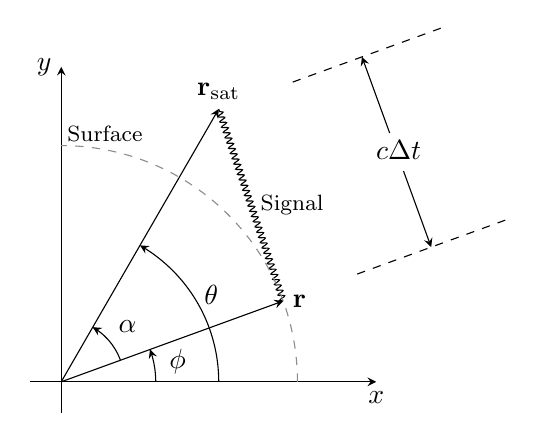
\begin{tikzpicture}[decoration = {snake,pre length=0pt,post length=0pt,amplitude=0.4mm,segment length=2}]
\draw[>=stealth,->] (-0.4,0) -- (4.0,0) node [pos=1,below] {\(x\)};
\draw[>=stealth,->] (0,-0.4) -- (0,4.0) node [pos=1,left] {\(y\)};
\draw[>=stealth,->] (0,0) -- (20:3cm) node [pos=1,right] {\(\textbf{r}\)};
\draw[>=stealth,->] (0,0) -- (60:4cm) node [pos=1,above] {\(\textbf{r}_{\text{sat}}\)};
\draw[decorate] (20:3) -- (60:4) node [pos=0.5,right] {\footnotesize Signal};
\draw[dashed] (20:4) -- (20:6); 
\draw[dashed] (60:4) +(20:1) -- +(20:3);
\draw[>=stealth,<-] (20:5) -- +(20+90:{0.4*sqrt((4*cos(60)-3*cos(20))^2+(4*sin(60)-3*sin(20))^2)});
\draw[>=stealth,->] (20:5) 
+(20+90:{0.6*sqrt((4*cos(60)-3*cos(20))^2+(4*sin(60)-3*sin(20))^2)}) -- 
+(20+90:{1.00*sqrt((4*cos(60)-3*cos(20))^2+(4*sin(60)-3*sin(20))^2)});
\draw node at (34.5:5.2) {\(c\Delta t\)}; 
\draw[variable=\x, domain=0:20, smooth, samples=60, >=stealth, ->] plot (\x:1.2);
\draw node at (10:1.5) {\(\phi\)};
\draw[variable=\x, domain=20:60, smooth, samples=60, >=stealth, ->] plot (\x:0.8);
\draw node at (40:1.1) {\(\alpha\)};
\draw[variable=\x, domain=0:60, smooth, samples=60, >=stealth, ->] plot (\x:2.0);
\draw node at (30:2.2) {\(\theta\)};
\draw[black!45!white, dashed, variable=\x, domain=0:90, smooth, samples=45] plot (\x:3);
\draw node at (80:3.2) {\footnotesize Surface};  
\end{tikzpicture}}
\caption{An illustration of the GPS exercise.}
\label{fig:GPS}
\end{figure}






\item Now comes the fun part. We want to find our own position on the planet. We will use figure \ref{fig:GPS} as a guide.
\\
We define the two following vectors: a satellite's position with respect to the center of the Earth, $\textbf{r}_{\text{sat}}$, and our position with respect to the center of the Earth, $\textbf{r}$. These two vectors can be given as

\begin{align*}
\textbf{r}_{\text{sat}}=\begin{bmatrix}x_{\text{sat}}\\y_{\text{sat}}\end{bmatrix} &&\text{and}&& \textbf{r}=\begin{bmatrix}x\\y\end{bmatrix},
\end{align*}

where $x_{\text{sat}}$ and $x$ is the $x$-position of the satellite and us respectively, and $y_{\text{sat}}$ and $y$ is the $y$-position of the satellite and us respectively. The satellites' positions are known, but only the length of our position vector is known, $|\textbf{r}|=r_{\text{Earth}}$. Hence we need some trigonometric properties to find our position.
\\
If we knew the angles $\alpha$ and $\theta$ in figure \ref{fig:GPS}, it would be easy to find our position. You should remember from the law of cosine from highschool (which is valid for any triangle):

\begin{equation}
C^{2}=A^{2}+B^{2}-AB\cos{\alpha}
\end{equation}

Using the law of cosine on the triangle created by $|\textbf{r}_{\text{sat}}|$, $|\textbf{r}|$ and $|\textbf{r}_{\text{sat}}-\textbf{r}|$ we find (notice in figure \ref{fig:GPS} that $|\textbf{r}_{\text{sat}}-\textbf{r}|=c\Delta t$)

\begin{align*}
(c\Delta t)^{2}&=|\textbf{r}_{\text{sat}}-\textbf{r}|^{2}=|\textbf{r}|^{2}+|\textbf{r}_{\text{sat}}|^{2}-2|\textbf{r}||\textbf{r}_{\text{sat}}|\cos{\alpha}\\
\alpha&=\arccos{\left(\frac{|\textbf{r}|^{2}+|\textbf{r}_{\text{sat}}|^{2}-(c\Delta t)^{2}}{2|\textbf{r}||\textbf{r}_{\text{sat}}|}\right)}
\end{align*}

We can now insert numbers to find the angle $\alpha$.
\\
Next we wanted to know the angle $\theta$. The definition of tangent is

\begin{align*}
\tan{\theta}=\frac{y_{\text{sat}}}{x_{\text{sat}}} \Rightarrow \theta=\arctan{\left(\frac{y_{\text{sat}}}{x_{\text{sat}}}\right)}
\end{align*}

Again, we insert numbers to find the value of the angle $\theta$. \textbf{FORKLAR hvilken vinkel man skal bruke}
\\
Figure \ref{fig:GPS} tells us that $\phi=\theta-\alpha$. To find our position we use the definition of sine and cosine:

\begin{align*}
\cos{\phi}&=\frac{x}{|\textbf{r}|} &&\Rightarrow&& x=|\textbf{r}|\cos{\phi}\\
\sin{\phi}&=\frac{y}{|\textbf{r}|} &&\Rightarrow&& y=|\textbf{r}|\sin{\phi}
\end{align*}

We insert numbers to find our position (check $\ldots$ for solution).
%\begin{align*}
%\vec{r}_{\text{sat}}=\begin{vmatrix}x_{\text{sat}}\\y_{\text{sat}}\end{vmatrix} &&\text{and}&& \vec{r}=\begin{vmatrix}x\\y\end{vmatrix} &&\Rightarrow&& \vec{r}_{\text{sat}}-\vec{r}=\begin{vmatrix}x_{\text{sat}}-x\\y_{\text{sat}}-y\end{vmatrix}
%\end{align*}
%|vec{r}_{\text{sat}}-\vec{r}|^{2}=(x_{\text{sat}}-x)^{2}+(y_{\text{sat}}-y)^{2}

\item In the deduction above we made a fatal error. We assumed that $|\textbf{r}_{\text{sat}}-\textbf{r}|=c\Delta t$. Here we assumed that $\Delta t=t_{\text{Earth}}-t_{\text{sat}}$, where $t_{\text{sat}}$ is the time the satellite sent out the signal and $t_{\text{Earth}}$ is the time when we recived the signal. Here we have not taken relativistic effects into account, thus we should get a wrong answer.
\\
We therefore need to find an the actual time that the light uses to reach us. We will use the same method as in the lecture note and in exercise 2C.7. It will therefore be a much shorter explenation here.

\begin{align*}
\Delta t_{\text{sat}}^{2}&=\Delta (s^{\prime})^{2}=\left(1-\frac{2M}{|\textbf{r}_{\text{sat}}|}\right)\Delta t^{2}-\frac{\overbrace{\Delta r^{2}}^{=0}}{1-\frac{2M}{|\textbf{r}_{\text{sat}}|}}-|\textbf{r}_{\text{sat}}|^{2}\Delta\theta^{2}_{\text{sat}}\\
&=\left(1-\frac{2M}{|\textbf{r}_{\text{sat}}|}\right)-|\textbf{r}_{\text{sat}}|^{2}\frac{\Delta\theta^{2}_{\text{sat}}}{\Delta t^{2}}=1-\frac{2M}{|\textbf{r}_{\text{sat}}|}-v_{\text{sat}}^{2}
\end{align*}

\begin{align*}
\Delta t_{\text{earth}}^{2}&=\Delta s^{2}=\left(1-\frac{2M}{|\textbf{r}|}\right)\Delta t^{2}-\frac{\overbrace{\Delta r^{2}}^{=0}}{1-\frac{2M}{|\textbf{r}|}}-r^{2}\Delta\phi^{2}_{\text{earth}}\\
&=\left(1-\frac{2M}{|\textbf{r}|}\right)-|\textbf{r}|^{2}\frac{\Delta\phi^{2}_{\text{earth}}}{\Delta t^{2}}=1-\frac{2M}{|\textbf{r}|}-v_{\text{earth}}^{2}
\end{align*}

\begin{equation*}
\frac{\Delta t_{\text{sat}}}{\Delta t_{\text{earth}}}=\sqrt{\frac{1-\frac{2M}{|\textbf{r}_{\text{sat}}|}-v_{\text{sat}}^{2}}{1-\frac{2M}{|\textbf{r}|}-v_{\text{earth}}^{2}}}
\end{equation*}

\item (Check $\ldots$ for solution)

\item (Check $\ldots$ for solution)

\item The more time that passes, the more wrong the expression $|\textbf{r}_{\text{sat}}-\textbf{r}|=c\Delta t$ becomes since $\Delta t$ is wrong. After a couple of days, the GPS will be totaly useless and just give wrong positions.

\end{enumerate}


\end{document}
